\documentclass[preprint,12pt]{article}

\usepackage{algorithmic}
\usepackage{algorithm}
\usepackage{enumerate}
\usepackage{enumitem}
\usepackage{graphics}
\usepackage{graphicx}
\usepackage{geometry}
\usepackage{amsmath}
\usepackage{wrapfig}
\usepackage{subfig}
\usepackage{framed}
\usepackage{color}
\usepackage{soul}
\usepackage{bm}

\usepackage{natbib}
\usepackage{multirow}
\usepackage[T1]{fontenc}
\usepackage[latin9]{inputenc}
%\usepackage{units}
\usepackage{esint}
\geometry{legalpaper,  margin=1in}

\newcommand{\CM}[2][green]{ {\sethlcolor{#1} \hl{#2}} }
\newcommand{\KB}[2][cyan]{ {\sethlcolor{#1} \hl{#2}} }
%THIS IS TO PUT ALL FLOATS AT THE END OF THE DOC SO THEY CAN BE SPLIT INTO A SEPARATE FILE
%%\usepackage{endfloat}
%\makeatother

%\usepackage{babel}

\begin{document}
\title{An Empirical Bayesian Framework for Assessing Partisan Bias in Redistricting Plans}

\author{Kevin Baas and Colin McAuliffe}

\maketitle

\begin{abstract}
There are several legal and technical challenges to the establishment of a standard for limiting partisan gerrymandering, and a few methods have been proposed thus far.
All methods for examining gerrymandering use observations of the results of one or more elections to make inferences about the tendency of a given redistricting plan to lead to biased outcomes.  
Here we propose an empirical Bayesian framework which allows an analyst to make such inferences accurately by using all available election results for the redistricting plan in question in a robust and consistent statistical model.
The framework can be used with any gerrymandering metric.

Keywords: Redistricting, gerrymander, Whitford v. Gill, 

\end{abstract}

\section{Introduction}
In the United States, the process of drawing districts for a state's legislative bodies and federal congressional delegation is usually in the hands of that state's legislature.
Partisan state legislatures have used the redistricting process in pursuit of various goals such as incumbent protection, maximizing their share of seats, and even diluting the voting power of citizens on the basis of race.
Opportunities to manipulate the redistricting process for partisan advantage abound, particularly with the advent of sophisticated algorithms for redistricting as well as a high degree of partisan and geographic polarization in the current political climate.
However, the Supreme Court has yet to rule definitively on the issue of partisan gerrymandering, and recent rulings suggest that a manageable standard for measuring gerrymandering is a prerequisite for a such a ruling (LULAC v. Perry 2004).

The establishment of some standards to reel in partisan gerrymandering would have significant consequences for democracy in the United States.
Partisan gerrymandering not only distorts the composition of legislative bodies, it represents a dilution of the voter's ability to attempt to influence policy by electing representatives of their choosing.
The ability of state legislatures to use redistricting to influence the outcome of elections comes at the direct expense of voter's ability to use their ballot to influence the outcome of elections.
However, in order to properly asses the harm caused by partisan gerrymandering, courts require mathematical tools for analyzing partisan bias in a redistricting plan.

The empirical Bayesian framework that we propose is not only appropriate for assessing bias that has existed in past redistricting plans, but it is useful for understanding how bias could be introduced into future redistricting plans, even as strategies for gerrymandering change in response to the introduction of a hypothetical standard.
In fact, the empirical Bayesian model that we propose is compatible with all metrics, and can be used as part of a standard itself, or can be used to test the robustness of standards that do not require Monte Carlo simulation. 
We therefore contend that regardless of whether or not the approach we present is an acceptable judicial standard itself, it remains a powerful tool for assessing partisan bias in redistricting plans that will prove useful for researchers and advocates of redistricting reform.
For example, the Monte Carlo technique can be used to evaluate the properties of metrics which do not have well known analytic statistical properties such or to evaluate the effect of the IID assumption for metrics which do have known analytic properties such as the mean median difference and the t-test.
Additionally, the technique could be used to help develop an understanding of the conditions where different metrics may agree or disagree with one another.


\section{Modeling the Likelihood of Bias in Future Elections\label{sec:FB}}

We can measure bias in a single election with the specific asymmetry, but we would also like to know the chances that a given redistricting plan will lead to bias in future elections.
This allows us to distinguish between chance occurrences of asymmetry on an otherwise fair map and maps for which asymmetry is a persistent feature.
A particular election result represents one possible outcome among many outcomes that could have occurred, or in other words each election represents a sample from a population representing all possible election outcomes.
We can use the observation of one or more elections along with prior knowledge of election data to make inferences about the population.
To this end we estimate parameters for a statistical model representing partisanship in each district as well as statewide partisanship, given at least one election result in a state.
Each sample drawn from this model represents a plausible election result that could have occurred if we were able to rerun elections as many times as we wanted.
Because we are using Monte Carlo integration, each sample is drawn with probability proportional to its empirical likelihood according to the model.
Thus, to get the expected specific asymmetry we simply take the average specific asymmetry of all samples drawn.
We also use these draws to calculate other descriptive statistics representing the likelihood of different levels of asymmetry.
A schematic illustration of the process is shown in figure \ref{fig:ProbModel}
Thus, the proposed definition that \emph{a fair redistricting plan is one that, on average, will not be biased in favor of either of the two major parties} corresponds to a map with an expected asymmetry of zero.
The details of the empirical Bayesian model are outlined in what follows.

\begin{figure}[htb!]
    \begin{center}
        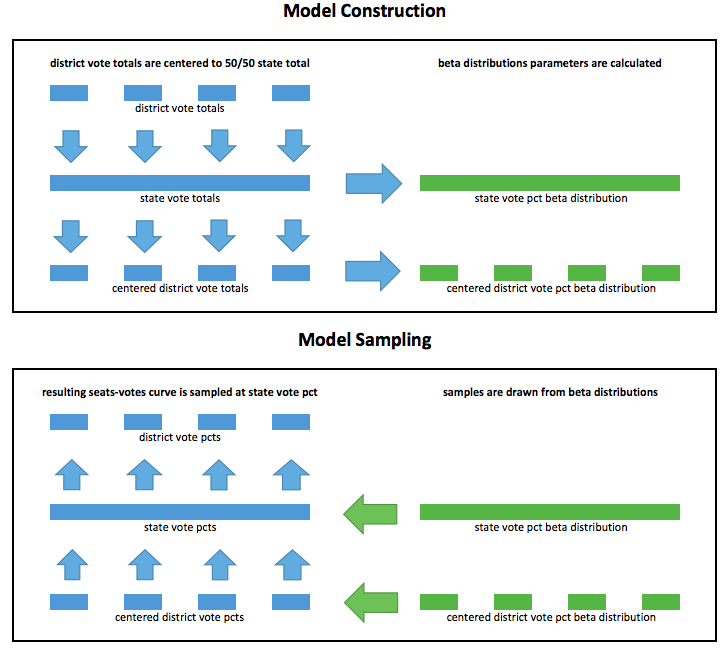
\includegraphics[scale=0.6]{../../Figures/Other/probability_model.png}
        \caption{Schematic illustration of empirical Bayesian probability model}\label{fig:ProbModel}
    \end{center}
\end{figure}
\subsection{Model Parameterization}
To chose a model appropriately, we must carefully consider the underlying process. 
The Beta distribution is a natural choice for many processes that involve percentages, and is appropriate for modeling election outcomes. 
This choice of probability model for modeling an election has been used in numerous academic papers, and continues to be used in literature published quite recently \cite{Paolino_2001_,Kaplan_2003_10.1287/opre.51.1.32.12794,Murr_2015_10.1177/2053168015583346}.
Indeed, teaching materials about the Beta distribution often use elections as an example.  
Some academic papers have extended this model to take into account third parties by using the Dirichlet distribution \cite{Rigdon_2009_10.1177/1532673X08330670} (The Dirichlet distribution is the multivariate extension of the Beta distribution.) 

The choice of the Beta distribution follows from first principles. 
In fact, two different points of view of the underlying stochastic process of election results both lead us to the Beta distribution. 
In the first point of view, we can consider the underlying stochastic process is a Bernoulli process; a number of trials that can each have one of two outcomes, i.e. a Republican vote or a Democratic vote.
We are interested in the number of votes for a given party out of all the votes, which is the number of successes in a sequence of trials.  
This leads us to the Binomial distribution. 
However, we do not know the rate of 'successes' (or the votes for an arbitrarily selected party), that is what we are trying to estimate.  
To estimate the rate parameter of a Binomial distribution, we use its conjugate prior distribution, which is the Beta distribution.

In the second perspective, voting is considered a pair of Poisson processes, which are series of events occurring at a certain rate i.e. voters for a party turning out to cast a vote. 
Here we are interested in the number of times a voter for a party turns out to vote in a given amount of time (Election day) - the number of events in a fixed interval. 
This leads us to the Poisson distribution.  
However, we do not know the \emph{rate} of events - that is what we are trying to estimate.  
To estimate the rate parameter of a Poisson distribution, we use its conjugate prior distribution, which is the Gamma distribution. 
To represent partisanship as a fraction, we take the fraction of events between the two Poisson processes.  
Let $\Gamma\left(X\right)$ be the unknown rate of voter turnout for one party, and $\Gamma\left(Y\right)$ the unknown rate for the other.
The proportion of votes won by party X is $\frac{\Gamma\left(X\right)}{\Gamma\left(X\right)+\Gamma\left(Y\right)} $. 
This leads us to the Beta distribution.

Thus, deduction from first principles leads us to select the Beta distribution as our probability model for the outcome of an election, regardless of which perspective we initially take.
With the choice of model parameterization in hand, we now turn our attention to estimation of the parameters for the Beta distributions.

\subsection{Parameter Estimation}
The shape parameters for the beta distributions for district partisanship are estimated using the method of moments as follows
\begin{equation}
    \alpha = \bar{x} \left(\frac{\bar{x}\left(1-\bar{x}\right)}{\bar{v}}-1\right)
\end{equation}
\begin{equation}
    \beta = \left(1-\bar{x}\right) \left(\frac{\bar{x}\left(1-\bar{x}\right)}{\bar{v}}-1\right)
\end{equation}
where $\bar{x}$ is the district mean vote percentage and $\bar{v}$ is the variance of the district vote percentage.
A practical challenge to using these formulas is that at most five data points will be available for a given district in a redistricting cycle.
Often, fewer data points may be available if a redistricting cycle is not yet complete or if a district had uncontested elections.
To make use of the model when only one data point is available and to help reduce the effects of small sample sizes in the parameter estimation process, we use a shrinkage term when computing the district variance $\bar{v}$ for N observed elections as follows

\begin{equation}
    \bar{v} = \frac{1}{N}\left[\sum_{n=1}^{N}\left(x_{n}-\bar{x}\right)^{2}+\hat{v}\right]
\end{equation}
where $\hat{v}$ is the shrinkage variance which can be set based on historical data.
Note that if there is only one data point available the variance is simply the shrinkage variance, without which the variance would be undefined.

To obtain $\hat{v}$, we use the average sample variance of district partisanship in contested elections over all districts and cycles.
This is show in figure \ref{fig:varHist}, where we obtain an average variance of .529\% (corresponding to a standard deviation of 7.26\%) over all cycles.
The within cycle average could also be used as the shrinkage variance, to attempt to capture trends in political polarization.

\begin{figure}[htb!]
    \begin{center}
        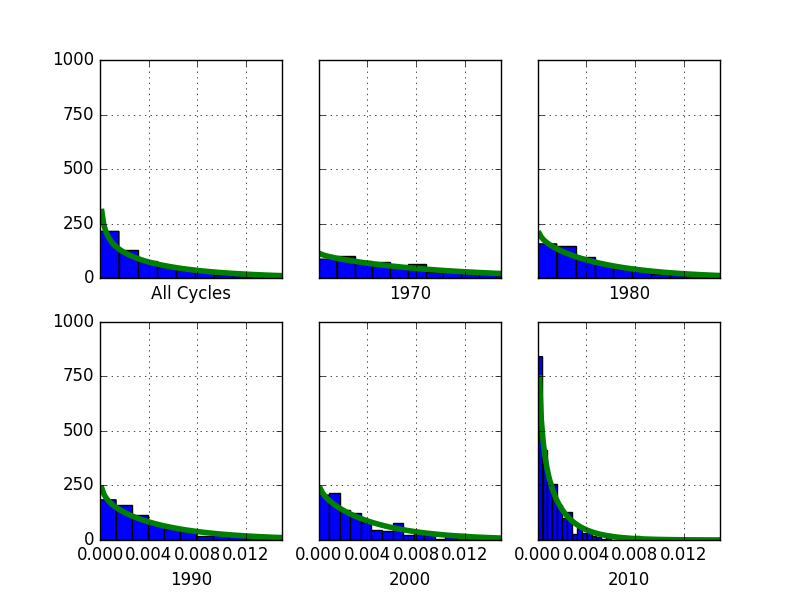
\includegraphics[scale=0.8]{../../Figures/HistoricAsymmetry/VarHist.png}
        \caption{Distribution of sample variance of district partisanship over contested elections in each cycle. The green lines are the result of fitting the variances to a beta distribution}\label{fig:varHist}
    \end{center}
\end{figure}
\subsection{Model Integration}
To compute the expected specific asymmetry, we use Monte Carlo sampling.
One sample from the model involves taking one sample from each district and one sample for the popular vote.
Seat counts can then be tallied along with various measures of bias and competitiveness.
We then compute the average specific asymmetry over all samples along with other descriptive statistics.
This approach has several advantages

\begin{itemize}

\item Non-uniform swings are accounted for. Accounting for the average partisanship of each district as well as the variance in partisanship from election to election captures the changes in voter sentiment that are not uniform throughout the state.

\item It takes into account all possibilities, weighted by likelihood - Every possible seats-votes curve and every possible popular vote ratio is taken into consideration, weighted by the combined likelihood of the two.

\item It shows durability - By computing an entire likelihood function for specific partisan asymmetry, rather than a single point estimate, this approach enables quick and accurate assessment of how durable a gerrymander is. This gives us insight into how much more harm it will cause in the future, including what the likelihood is that it will not cause harm.

\end{itemize}

To illustrate the process we show a few samples from this model for the Wisconsin state assembly districts in figure \ref{fig:SVAssembly2010} (a full analysis of this districting plan can be found in section \ref{sec:Wis}).
The dark line is the seats votes curve generated from sampling the partisanship in each district, while the dashed line in the reflection of this curve.
Discrepancies between these two lines represent asymmetries, which vary depending on the level of partisanship considered.
The vertical line is the statewide partisanship sampled from the state beta distribution, which determines the partisanship level that we measure the asymmetry at.

\begin{figure}[htb!]
    \begin{center}
        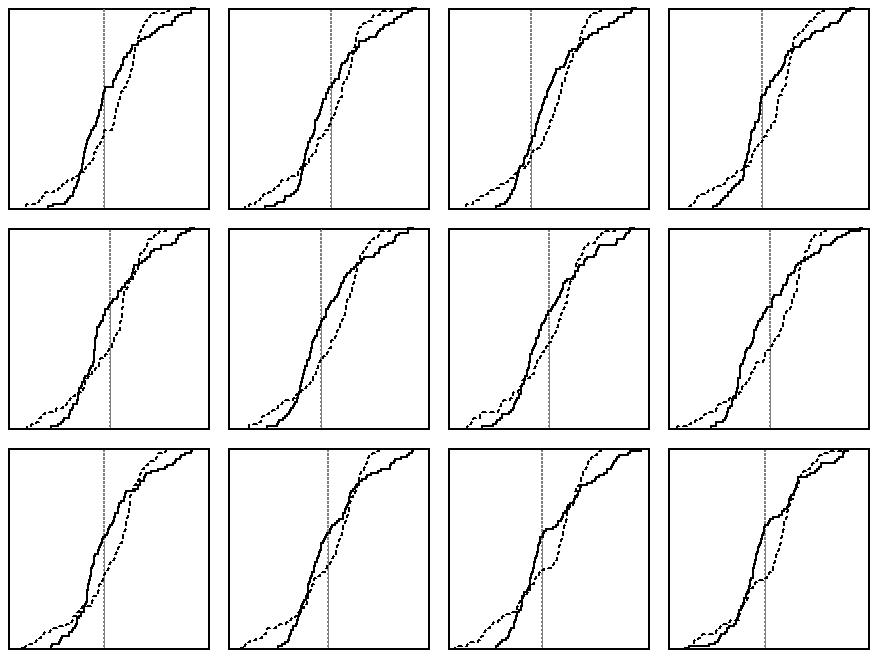
\includegraphics[scale=0.45]{../../Figures/WI2010/sv_curves_assembly.png}
        \caption{Some election outcome seats-votes curves generated from the probability model for Wisconsin 2010 Assembly districts}\label{fig:SVAssembly2010}
    \end{center}
\end{figure}


\clearpage
\section*{Acknowledgment}
\section*{}
\bibliographystyle{unsrt}
\bibliography{gerrymandering}
\clearpage



\end{document}
